% !TeX spellcheck = en_US

%TODO Sibel

	\begin{frame}{Smooth-Transition Model}
		\begin{block}{Smooth Transition} An infinitesimally small deformation that changes the topological relation between the line and the region
		\end{block}
		\begin{block}{Examples and Counterexamples}
			\centering
			\begin{tikzpicture}[->,>=stealth',shorten >=1pt,auto,node distance=4cm,
			thick]
			
			\node[rectangle] (1) {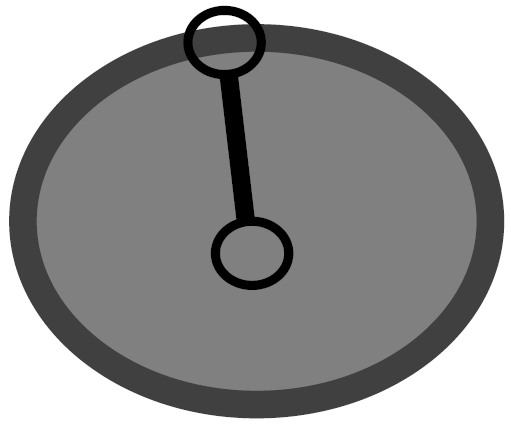
\includegraphics[width=2cm]{images/smooth_transitions_conceptual_neighborhood_3}};
			\node[rectangle] (2) [below left of=1] {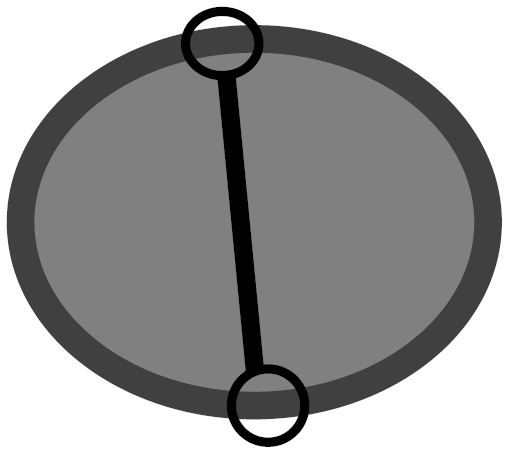
\includegraphics[width=2cm]{images/smooth_transitions_conceptual_neighborhood_1}};
			\node[rectangle] (3) [below right of=1] {
\includegraphics[width=2cm]{images/smooth_transitions_conceptual_neighborhood_2}};
			
			\path[every node/.style={font=\sffamily\small}]
				(1) edge node {} (2)
					edge node {\textcolor{green}{conceptual neighbors}} (3)
				(2) edge node {\textcolor{green}{conceptual neighbors}} (1)
					edge node {} (3)
				(3) edge node {} (1)
					edge node {\textcolor{red}{\begin{tabular}{c}
							\textbf{not} conceptual\\neighbors
							\end{tabular}}} (2);
			
%			(1) edge node [left] {0.6} (4)
%			edge [bend right] node[left] {0.3} (2)
%			edge [loop above] node {0.1} (1)
%			(2) edge node [right] {0.4} (1)
%			edge node {0.3} (4)
%			edge [loop left] node {0.4} (2)
%			edge [bend right] node[left] {0.1} (3)
%			(3) edge node [right] {0.8} (2)
%			edge [bend right] node[right] {0.2} (4)
%			(4) edge node [left] {0.2} (3)
%			edge [loop right] node {0.6} (4)
%			edge [bend right] node[right] {0.2} (1);
			\end{tikzpicture}
		\end{block}
	\end{frame}
	\begin{comment}
	- second conceptual neighborhood model
	- smooth transition: definition
	- occurrence of smooth transition -> conceptual neighborhood
	\end{comment}
	
	
	\begin{frame}{Formalization}
		\begin{block}{A smooth transition occurs by moving around the line's}
		\begin{enumerate}
			\item \textbf{boundary nodes}\\ \vspace{6pt}
			\textbf{Q:} Do they intersect with the same region part?\\
			\Highlight{Transition Rule 1} \textbf{if} Yes\\
			\Highlight{Transition Rule 2} \textbf{if} No
			
			\item \textbf{interior}\\ \vspace{6pt}
			\Highlight{Transition Rule 3} \textbf{to} extend the intersection area \textit{and}\\
			\Highlight{Transition Rule 4} \textbf{to} reduce it
		\end{enumerate}
		\end{block}
		
		\begin{block}{What this means for the 9-intersection:}
			 An entry or its adjacent entries gets changed from \Empty{} to \NotEmpty{} or v.v.
		\end{block}
	\end{frame}
	\begin{comment}
	- if you do not understand, no pressure as this will be explained in more detail in the upcoming slides.
	\end{comment}
	
	\begin{frame}{One More Thing...}
		\begin{block}{Definition (Extent of a line part $i$)}
			\begin{itemize}
				\item Denoted by $\#M[i, \_]$
				\item Count of intersections betw. line part $i$ and the region parts
				\item $\#M[i, \_]$ in the interval $[0\dots 3]$
			\end{itemize}
		\end{block}
	\end{frame}
	\begin{comment}
	- we need to define this before we continue with the transition rules
	- extent of a line's interior with respect to a region is in the interval of 1 to 3
	- extent of the line's boundary is either 1 (if both nodes are located in the same region part) or 2 (if the nodes are located in different parts of the region)
	- extent of a line's interior is always 3
	- draw 9-intersection model on the board for reference
	\end{comment}
	
	\begin{frame}{Transition Rule 1}
		\begin{block}{}
			If the line's two boundaries intersect with the \Highlight{\textbf{same}} region part, then extend the intersection to either of the adjacent region parts:
		\end{block}
		\begin{block}{}
			\centering $ \#M[\delta, \_] = 1 \Highlight{\implies}
			\forall i (M[\delta, i] = \NotEmpty):
			M_{N}[\delta, \text{adjacent}(i)] := \NotEmpty $
		\end{block}
		\begin{block}{}
			%Moving one boundary of a line into an adjacent part of the region.
			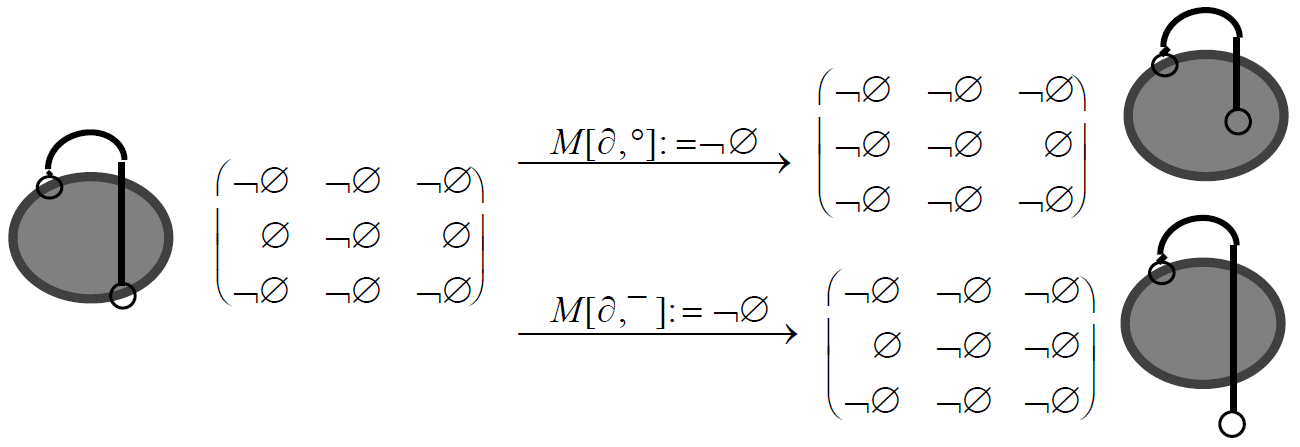
\includegraphics[width=\textwidth]{images/smooth_transitions_example_a.png}
		\end{block}
	\end{frame}
	\begin{comment}
		- Moving a line's boundary node from a region part into an adjacent part of the region.
	\end{comment}
	
	\begin{frame}{Transition Rule 2}
		\begin{block}{}
			If the line's two boundaries intersect with two \Highlight{\textbf{different}} region parts then move either intersection to the adjacent region part:
		\end{block}
		\begin{block}{}
			\centering $ \#M[\delta,\_] = 2 \Highlight{\implies}
			\forall i (M[\delta, i] = \NotEmpty):$
			$M_{N}[\delta, i] := \Empty \Highlight{{}\land{}}
			M_{N}[\delta, \text{adjacent}(i)] := \NotEmpty $
		\end{block}
		\begin{block}{}
			%Moving either boundary into an adjacent region part.
			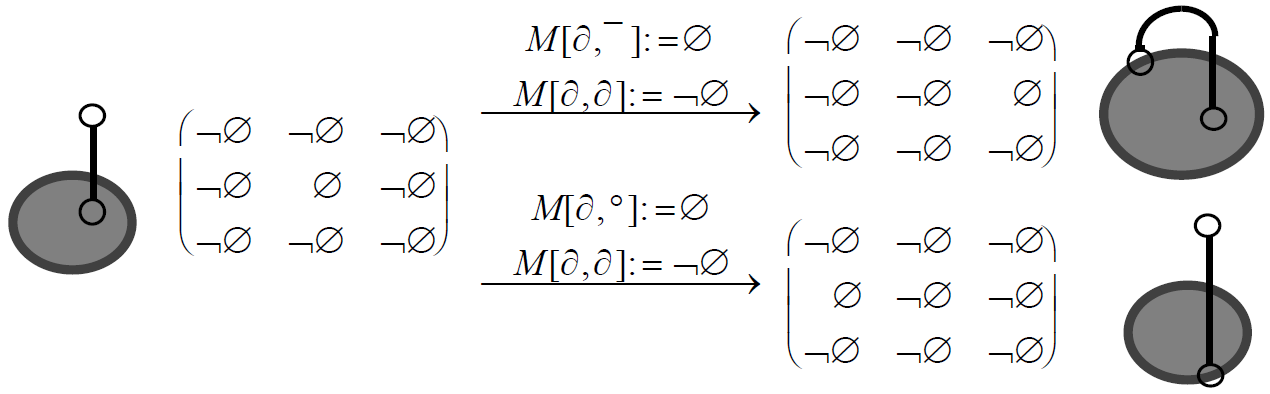
\includegraphics[width=\textwidth]{images/smooth_transitions_example_b.png}
		\end{block}
	\end{frame}
	\begin{comment}
		- Moving a line's interior-intersection to either of the adjacent region parts.
	\end{comment}
	
	\begin{frame}{Transition Rule 3}
		\begin{block}{}
			\Highlight{\textbf{Extend}} the line's interior-intersection to either of the adjacent region parts:
		\end{block}
		\begin{block}{}
			\centering $ \forall i (M[\textdegree, i] = \NotEmpty):
			M_{N}[\textdegree, \text{adjacent}(i)] := \NotEmpty $
		\end{block}
		\begin{block}{}
			%Moving the line's interior into an adjacent part of the region.
			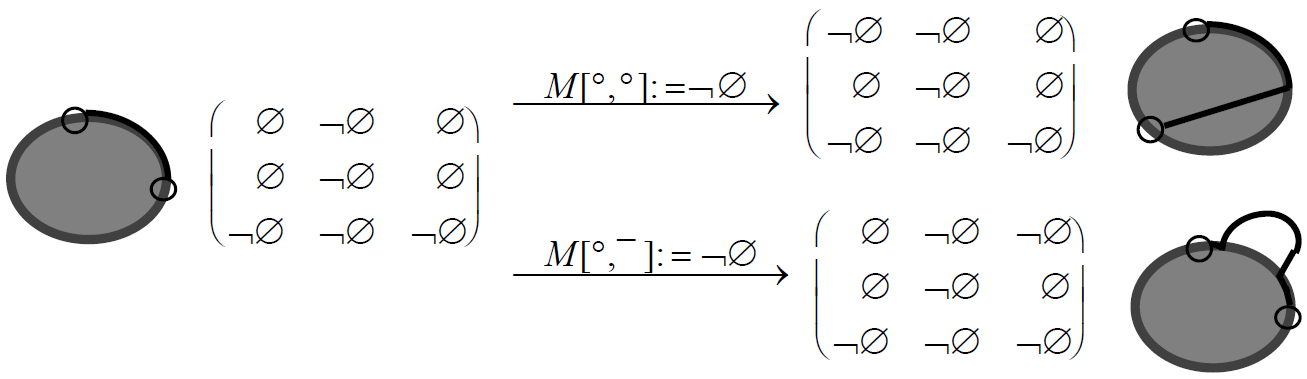
\includegraphics[width=\textwidth]{images/smooth_transitions_example_c.png}
		\end{block}
	\end{frame}
	
	\begin{frame}{Transition Rule 4}
		\begin{block}{}
			\Highlight{\textbf{Reduce}} the line's interior intersection on either of the adjacent region parts.
		\end{block}
		\begin{block}{}
			\centering
			$ \#M[\textdegree, \_] = 2 \Highlight{\implies}
			\forall i (M[\textdegree, i] = \NotEmpty):
			M_{N}[\textdegree, i] := \Empty $
			$ \#M[\textdegree, \_] = 3 \Highlight{\implies}
			\forall i (i \neq \delta):
			M_{N}[\textdegree, i] := \Empty $
		\end{block}
		\begin{block}{}
			%Moving the line's interior out of a part of the region.
			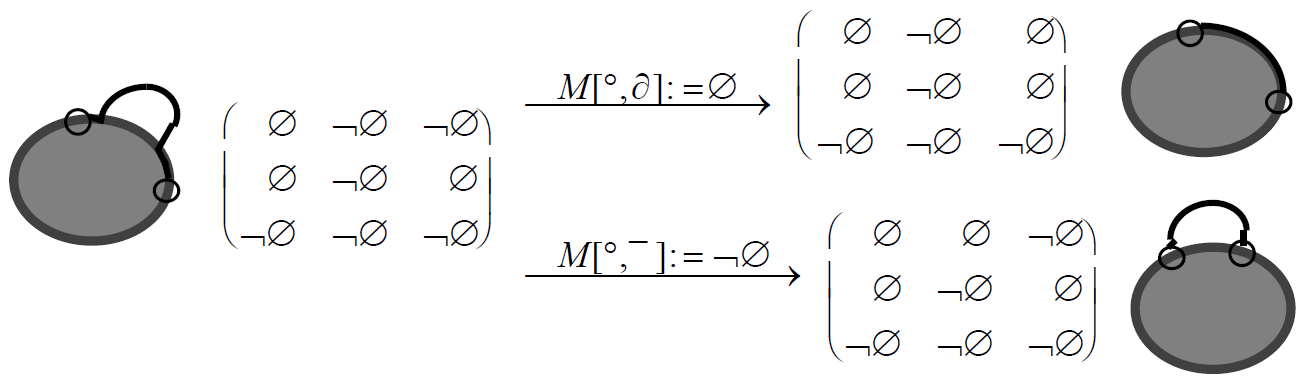
\includegraphics[width=\textwidth]{images/smooth_transitions_example_d.png}
		\end{block}
	\end{frame}
	
	\begin{frame}{Additional Consistency Constraints}
		\begin{enumerate}
			\item If the line's interior intersects with the region's interior \textit{and} exterior, then the line's interior must also intersect with the region's boundary.
			\\ \vspace{6pt}
			\begin{center}
				$ M[\textdegree,\textdegree] = \NotEmpty \Highlight{{}\land{}} M[\textdegree,^{-}] = \NotEmpty \Highlight{\implies} M[\textdegree,\delta] := \NotEmpty $
			\end{center}
			\item[ ]
			\item If the line's boundary intersects with the region's interior (exterior) then the line's interior must intersect with the region's interior (exterior) as well.
			\\ \vspace{6pt}
			\begin{center}
				$ M[\delta,\textdegree] = \NotEmpty \Highlight{\implies} M[\textdegree,\textdegree] := \NotEmpty $ \\
				$ M[\delta, ^{-}] = \NotEmpty \Highlight{\implies} M[\textdegree,^{-}] := \NotEmpty $
			\end{center}
		\end{enumerate}
		
	\end{frame}
	
	% NOTES:
	% The separate moves of the line's interior and boundaries are atomic operations that do not account for some of the properties of the objects and their embedding space and, therefore, may generate inconsistent 9-intersections for configurations that cannot be realized. In order to maintain connectivity among the line's boundaries and interior, it is necessary to assure the following \textbf{consistency constraint}: [1]. Likewise, in order to preserve the continuous-space property of $\mathcal{R}^{2}$, the following consistency constraint must be fulfilled: [2].
	
	\begin{frame}{Resulting Neighborhood Graph}
		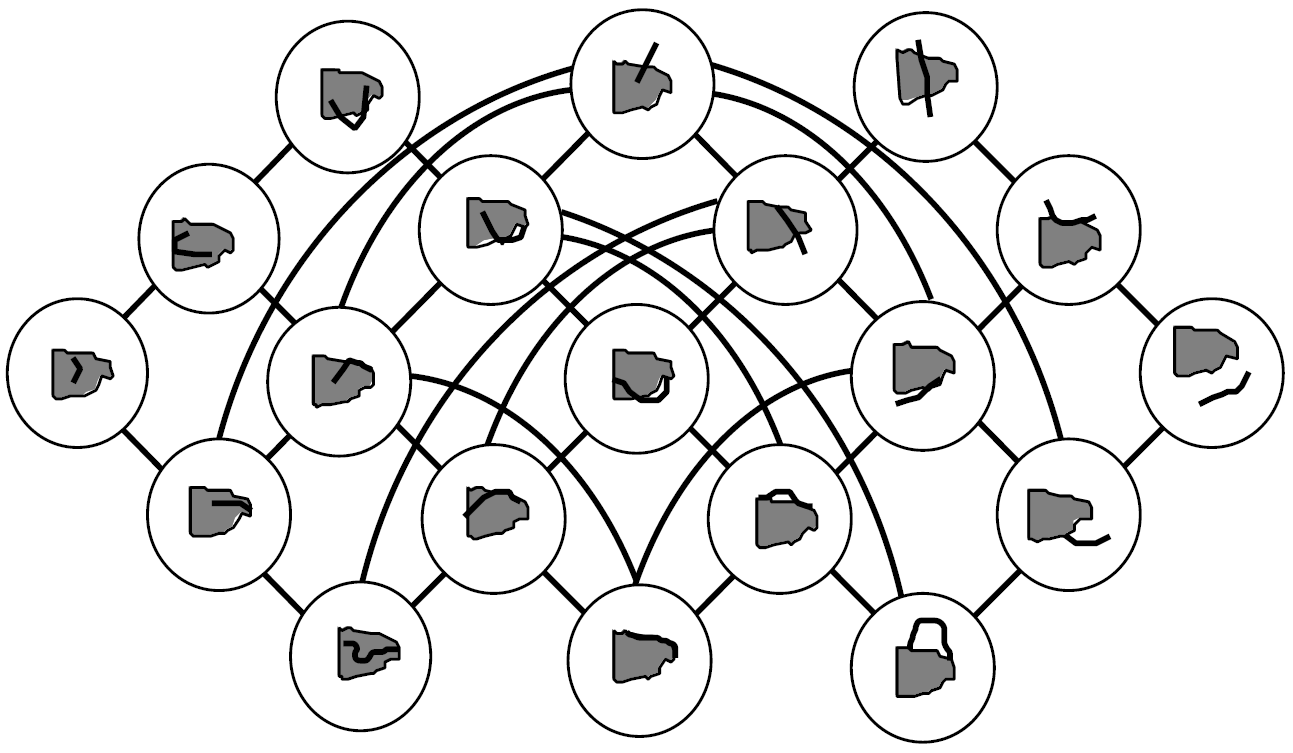
\includegraphics[width=\textwidth]{images/smooth_transitions_neighborhood_graph.png}
	\end{frame}
	\begin{comment}
		- all transition rules and constraints establish the smooth transitions for line-region relations
		- when applied to the 19 line-region relations, they provide this neighborhood graph
	\end{comment}
	
	\begin{frame}{Comparison}
		\begin{tabularx}{\textwidth}{XX}
			\begin{center}
				\textbf{Snapshot Model}
			\end{center}
			&
			\begin{center}
			\textbf{Smooth-Transition Model}
			\end{center} \\
			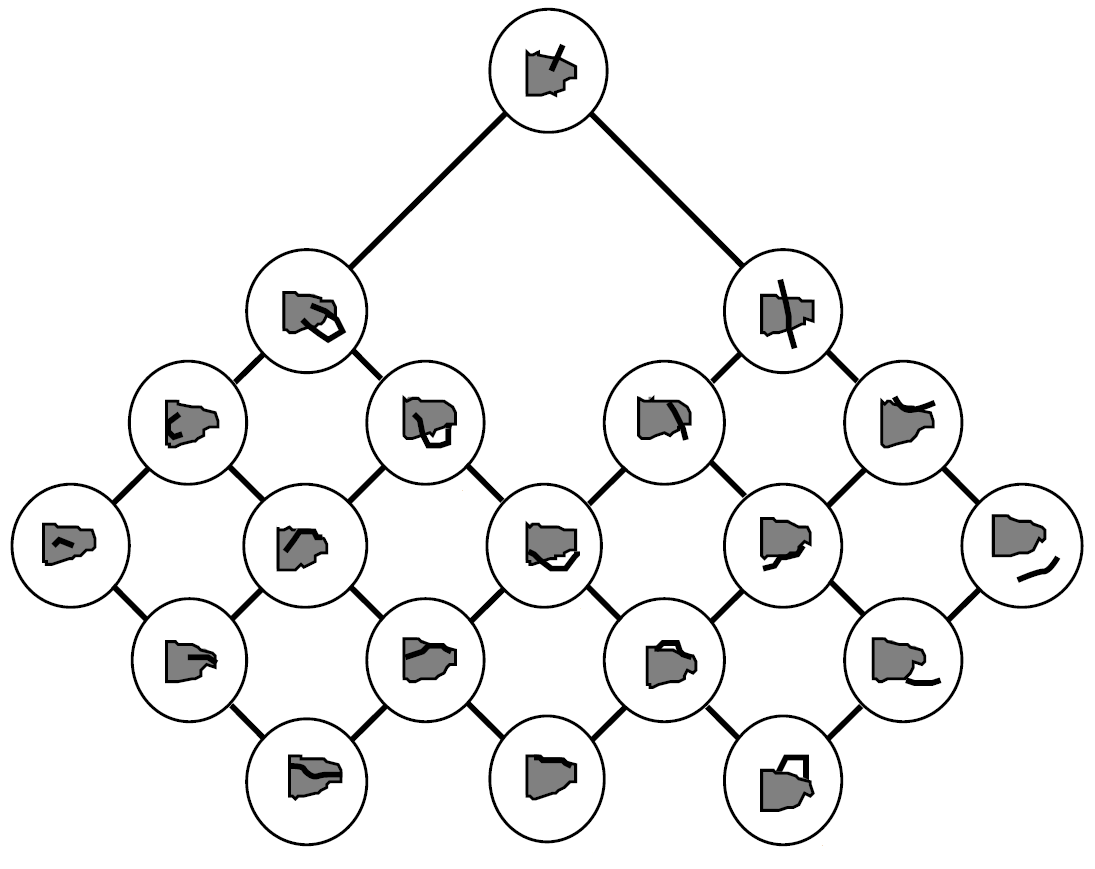
\includegraphics[width=0.48\textwidth]{images/snapshot_model_neighborhood_graph_simple.png}
			&
			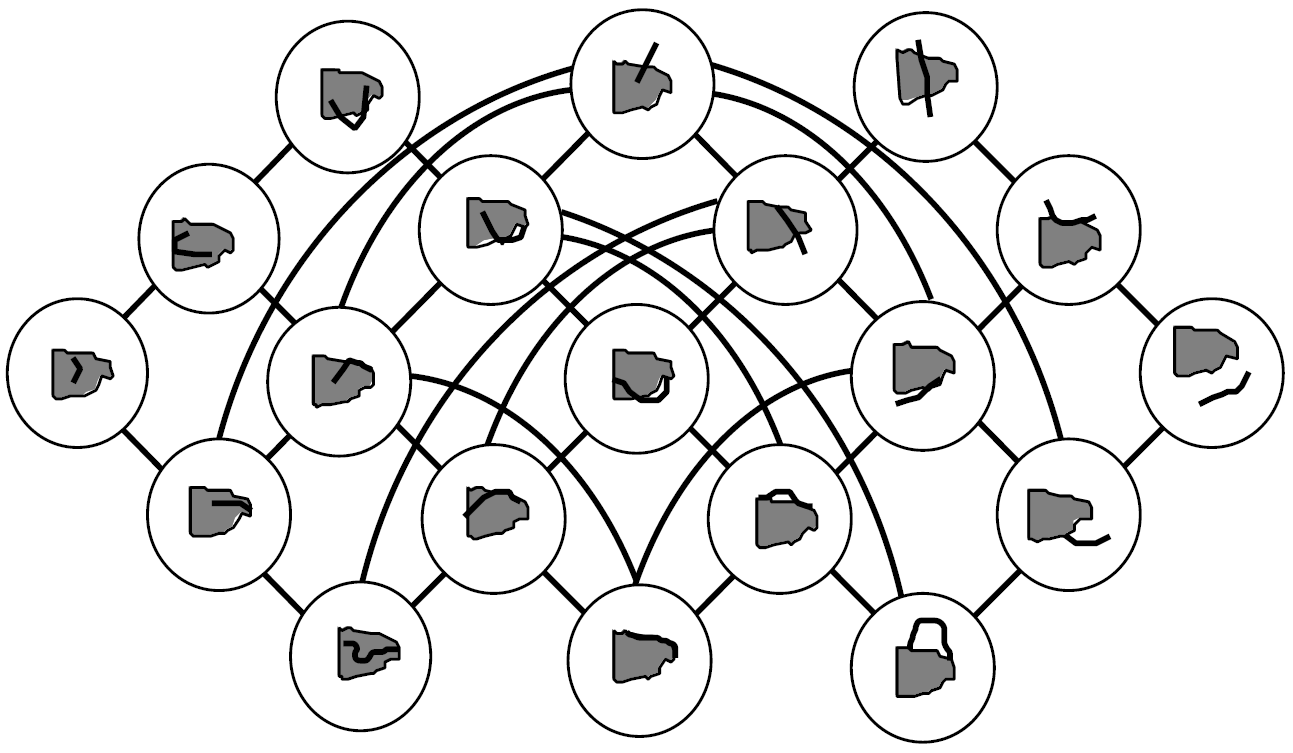
\includegraphics[width=0.48\textwidth]{images/smooth_transitions_neighborhood_graph.png}
		\end{tabularx}
	\end{frame}
	\begin{comment}
		- images are a bit small
		- the purpose is to give the audience just a feeling of how similar/ different the models are
		- resemble a lot in structure
		- differences are the way in which conceptual neighbors are connected at the to and the additional links that run across the smooth transition graph
		- 19 line-region relations $\rightarrow$ 171 distinct pairs of relations that can possibly be conceptual neighbors
		- 26 under snapshot model and the smooth-transition model
		- 2 under snapshot model
		- 12 under smooth-transition model
		- 131 pairs under neither model
		\end{itemize}
	\end{comment}